\chapter{Resultados}
\label{cap4}



\paragraph{} A partir dos parâmetros encontrados nas Seções anteriores, utilizou-se a seguinte configuração para encontrar a simulação com os melhores índices de performance:

\begin{itemize}
    \item 71 \textit{tickers} (Tabela \ref{tab:5})
    \item Período de simulação: 01/01/2019 a 31/12/2021
    \item Capital: R\$ 100000,00
    \item Período máximo de dias por operação: 45
    \item Risco de Entrada por Operação: 0,29
    \item Compensação por Lucratividade: Sim
    \item Descanso por Identificação de Crises: Sim
    \item Descanso por Tendência de Baixa: Sim
    \item RCC: 0,57\%
    \item Controle Proporcional para Uso de Capital (RCC Dinâmico): Sim
    \item Valor de Referência para Uso de Capital: 100\%
    \item Constante K de Ganho Proporcional: 14,5
\end{itemize}

\paragraph{} Os resultados encontrados podem ser verificados pela Tabela \ref{tab:13} e pela Figura \ref{fig:250}.

\begin{table}[h!] %ID 485
    \begin{center}
        \begin{tabular}{ l|c|c }
            Parâmetro & Estratégia & \textit{Baseline} \\
            \hline
            Rendimento Final & 124,59\% & 73,94\% \\
            Volatilidade & 37,70\% & 55,48\% \\
            Índice de Sharpe & 1,28 & 0,68 \\
            Índice de Sortino & 1,84 & 0,74 \\
            Correlação de Spearman (c/ \textit{Baseline}) & 0,89 & - \\
            Correlação de Spearman (c /Ibovespa) & 0,66 & - \\
            Uso Máximo de Capital & 100\% & 100\% \\
            Uso Médio de Capital & 91,46\% & 100\% \\
            Máximo de Operações Ativas & 64 & - \\
            Média de Operações Ativas & 35,15 & - \\
            Desvio Padrão de Operações Ativas & 16,53 & -\\
            Operações Totais & 1916 & 71 \\
            Operações de Sucesso & 565 (29,5\%) & - \\
            Operações de Falha & 1238 (64,6\%) & - \\
            Operações de \textit{Timeout} & 89(4,6\%) & - \\
            Operações Incompletas & 24(1,3\%) & - \\
        \end{tabular}
        \caption{Resultado final}
        \label{tab:13}
    \end{center}
\end{table}

\begin{figure}[!htb]
    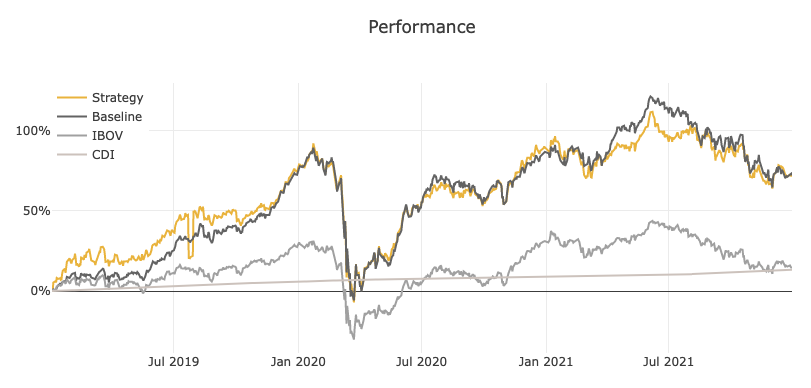
\includegraphics[scale=0.50]{performance_final.png}
    \centering
    \caption{Performance final}
    \label{fig:250}
\end{figure}
